%
% This is the LaTeX template file for lecture notes for EE 382C/EE 361C.
%
% To familiarize yourself with this template, the body contains
% some examples of its use.  Look them over.  Then you can
% run LaTeX on this file.  After you have LaTeXed this file then
% you can look over the result either by printing it out with
% dvips or using xdvi.
%
% This template is based on the template for Prof. Sinclair's CS 270.

\documentclass[twoside]{article}
\usepackage{graphicx}
\usepackage{csquotes}
\MakeOuterQuote{"}
\usepackage{lscape}
\usepackage{wrapfig}
\usepackage{amsmath}
\usepackage{amssymb}
\usepackage{listings}
\usepackage{algorithm}
\usepackage{algpseudocode}
\setlength{\oddsidemargin}{0.25 in}
\setlength{\evensidemargin}{-0.25 in}
\setlength{\topmargin}{-0.6 in}
\setlength{\textwidth}{6.5 in}
\setlength{\textheight}{8.5 in}
\setlength{\headsep}{0.75 in}
\setlength{\parindent}{0 in}
\setlength{\parskip}{0.1 in}

%
% The following commands set up the lecnum (lecture number)
% counter and make various numbering schemes work relative
% to the lecture number.
%
\newcounter{lecnum}
\renewcommand{\thepage}{\thelecnum-\arabic{page}}
\renewcommand{\thesection}{\thelecnum.\arabic{section}}
\renewcommand{\theequation}{\thelecnum.\arabic{equation}}
\renewcommand{\thefigure}{\thelecnum.\arabic{figure}}
\renewcommand{\thetable}{\thelecnum.\arabic{table}}

%
% The following macro is used to generate the header.
%
\lstset{language=Python, numbers=left, tabsize=2, xleftmargin=5.0ex}

\newcommand{\lecture}[4]{
   \pagestyle{myheadings}
   \thispagestyle{plain}
   \newpage
   \setcounter{lecnum}{#1}
   \setcounter{page}{1}
   \noindent
   \begin{center}
   \framebox{
      \vbox{\vspace{2mm}
    \hbox to 6.28in { {\bf EE 382V: Parallel Algorithms
                        \hfill Summer 2017} }
       \vspace{4mm}
       \hbox to 6.28in { {\Large \hfill Lecture #1: #2  \hfill} }
       \vspace{2mm}
       \hbox to 6.28in { {\it Lecturer: #3 \hfill Scribe: #4} }
      \vspace{2mm}}
   }
   \end{center}
   \markboth{Lecture #1: #2}{Lecture #1: #2}
   %{\bf Disclaimer}: {\it These notes have not been subjected to the
   %usual scrutiny reserved for formal publications.  They may be distributed
   %outside this class only with the permission of the Instructor.}
   \vspace*{4mm}
}

%
% Convention for citations is authors' initials followed by the year.
% For example, to cite a paper by Leighton and Maggs you would type
% \cite{LM89}, and to cite a paper by Strassen you would type \cite{S69}.
% (To avoid bibliography problems, for now we redefine the \cite command.)
% Also commands that create a suitable format for the reference list.
\renewcommand{\cite}[1]{[#1]}
\def\beginrefs{\begin{list}%
        {[\arabic{equation}]}{\usecounter{equation}
         \setlength{\leftmargin}{2.0truecm}\setlength{\labelsep}{0.4truecm}%
         \setlength{\labelwidth}{1.6truecm}}}
\def\endrefs{\end{list}}
\def\bibentry#1{\item[\hbox{[#1]}]}

%Use this command for a figure; it puts a figure in wherever you want it.
%usage: \fig{NUMBER}{SPACE-IN-INCHES}{CAPTION}
\newcommand{\fig}[3]{
			\vspace{#2}
			\begin{center}
			Figure \thelecnum.#1:~#3
			\end{center}
	}
% Use these for theorems, lemmas, proofs, etc.
\newtheorem{theorem}{Theorem}[lecnum]
\newtheorem{lemma}[theorem]{Lemma}
\newtheorem{proposition}[theorem]{Proposition}
\newtheorem{claim}[theorem]{Claim}
\newtheorem{corollary}[theorem]{Corollary}
\newtheorem{definition}[theorem]{Definition}
\newenvironment{proof}{{\bf Proof:}}{\hfill\rule{2mm}{2mm}}

% **** IF YOU WANT TO DEFINE ADDITIONAL MACROS FOR YOURSELF, PUT THEM HERE:

\begin{document}
%FILL IN THE RIGHT INFO.
%\lecture{**LECTURE-NUMBER**}{**DATE**}{**LECTURER**}{**SCRIBE**}
\lecture{22}{July 22}{Vijay Garg}{Michael Spagon}
%\footnotetext{These notes are partially based on those of Nigel Mansell.}















% **** YOUR NOTES GO HERE:

% Some general latex examples and examples making use of the
% macros follow.  
%**** IN GENERAL, BE BRIEF. LONG SCRIBE NOTES, NO MATTER HOW WELL WRITTEN,
%**** ARE NEVER READ BY ANYBODY.

\section{Introduction}

This lecture covers \textbf{range minimum queries (RMQ)} and briefly touches the related problem of finding the \textbf{lowest common ancestor (LCA)} of a pair of nodes in a segmented tree. 

We started to discuss \textbf{tree contraction algorithms} but did not finish by the end of the lecture.






\section{Range Minimum Query (RMQ)}

Given a fixed array $A[0 \ ... \ n \text{-} 1]$ of $n$ elements, and two specified indices $i \leq j$, a \textbf{range minimum query (RMQ)} is used to find the \textit{position} of the minimum element between the two indices.

A range minimum query on array $A$ with the indices 2 and 7 would be denoted as $RMQ_{A}(2,7)$.

With respect to the array below, $RMQ_{A}(2,7) = 3$. The smallest element within the subarray $A[2 \ ... \ 7]$ is 1, and the element is in the third position of the array.

\begin{figure}[h]
\center
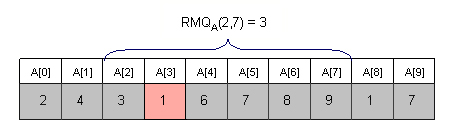
\includegraphics[scale=1]{rmq-example1.jpg}
\caption{Range minimum query on $A$ with index i = 2 and j = 7}
\end{figure}







\newpage
\subsection{A Na{\"i}ve Solution}

What if we precomputed all possible queries and stored the results in a data structure?

By creating a 2D array, $B$, such that $B[i,j] = min(A[i...j])$, a range min query can be solved in constant time $O(1)$ by array look-up in $B$.  Below is a look-up table for the RMQ's on a 10 element array $A$.

\begin{figure}[h]
\centering
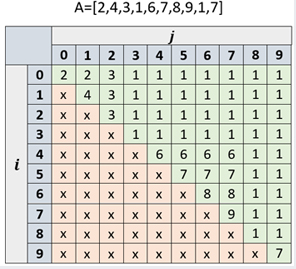
\includegraphics[width=0.5\textwidth]{lookup.jpg}
\caption{Look-up table for $RMQ_{A}(i,j)$}
\end{figure}

%Figure 2. Look-up table for RMQ_{A}(i,j)

As you can see this wastes a lot of space and is impractical for very large $n$: There are $O(n^2)$ possible queries for a length-$n$ array and therefore $O(n^2)$ entries for B.



\subsection{A Better Solution}
\textit{\textbf{Intuition:}} Instead of storing all possible ranges of indices, we should only store ranges that are a power of 2 ($i.e.$, $i = 2^a$ $j = 2^b$ where $a \leq b$.)

In this solution we will be using segmented trees and calculating the least common ancestor of two nodes within the tree, so we must discuss them first.


\newpage
{\large \textbf{Segmented Tree}}

We will use a \textbf{segmented tree}, a structure for storing intervals, where:
\begin{enumerate}
  \item Leaf nodes are the elements of array $A$.
  \item Each internal node is labeled with indices $i,j$ that represent information about the sub\textbf{segment} $A[i,j]$.  Each internal node stores two additional arrays $P$ and $S$ that represent the prefix and suffix minima, respectively.
\end{enumerate}

Below is a picture of a segmented tree that stores data that will help us perform RMQs on array $A$ = [3,1,5,7,2,8,6,4].  Notice that for this problem the array index starts at \texttt{1}.

\begin{figure}[h]
\centering
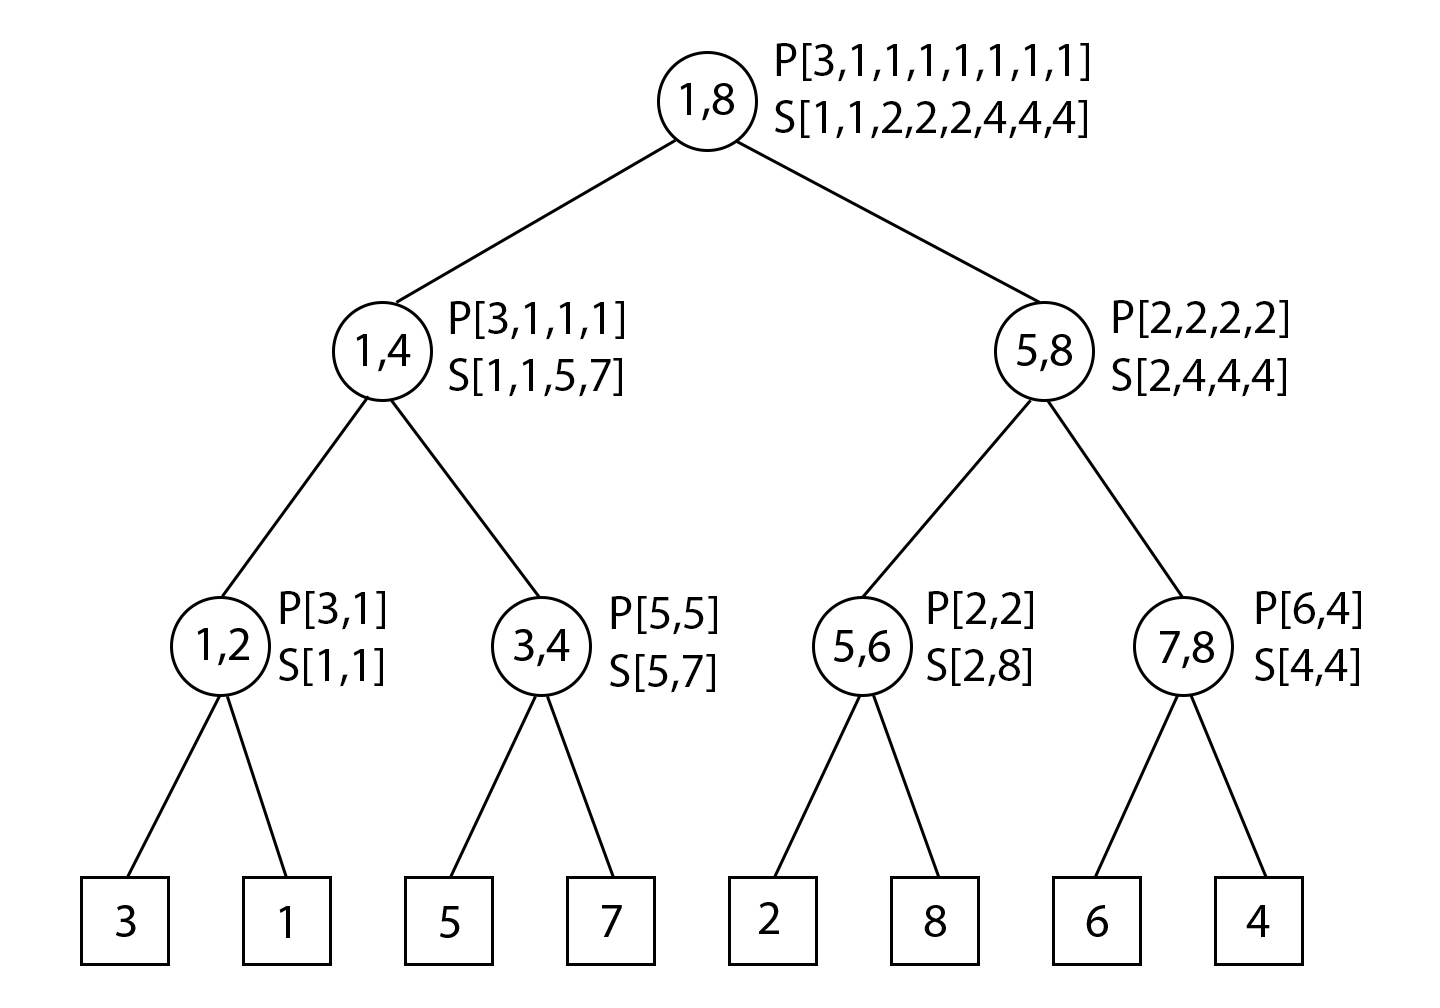
\includegraphics[width=1\textwidth]{tree.jpg}
\caption{A segmented tree used for range minimum query}
\end{figure}


\newpage

{\large \textbf{Prefix Minima Array}}

A \textbf{prefix minima} array \textbf{$P$} stores the current minimum value seen while traversing the input array from \textit{left} to \textit{right}.

For example, the internal node labeled "1,4" is associated with the subarray with indices $i=1$ and $j=4$. Therefore the input to \texttt{prefix minima} is $A[1,4] = [3,1,5,7]$. 
\begin{itemize}
  \item $P[1] = min(A[1,1]) = min(3) = 3$
  \item $P[2] = min(A[1,2]) = min(3,1) = 1$
  \item $P[3] = min(A[1,3]) = min(3,1,5) = 1$
  \item $P[4] = min(A[1,4]) = min(3,1,5,7) = 1$
\end{itemize}

The $P$ array contains [3,1,1,1] since the minimum value in $A[1,1]$ is 3; the minimum value in $A[1,2]$ is 1; the minimum value from $A[1,3]$ is 1; the minimum value from $A[1,4]$ is 1.

\hspace{5pt}

{\large \textbf{Suffix Minima Array}}

A \textbf{suffix minima} array \textbf{$S$} stores the current minimum value seen while traversing the input array from \textit{right} to \textit{left}.

For example, the internal node labeled "1,4" is associated with the subarray with indices $i=1$ and $j=4$. Therefore the input to \texttt{suffix minima} is $A[1,4] = [3,1,5,7]$. Remember this time we calculate the minimum from \textit{right} to \textit{left}.
\begin{itemize}
  \item $S[1] = min(A[4,4]) = min(7) = 7$
  \item $S[2] = min(A[4,3]) = min(7,5) = 5$
  \item $S[3] = min(A[4,2]) = min(7,5,1) = 1$
  \item $S[4] = min(A[4,1]) = min(7,5,1,3) = 1$
\end{itemize}


The $S$ array contains [7,5,1,1] since the minimum value in $A[4,4]$ is 7; the minimum value in $A[4,3]$ is 5; the minimum value in $A[4,2]$ is 1; the minimum value in $A[4,1]$ is 1.


\vspace{20pt}

\newpage
{\large \textbf{Least Common Ancestor}}

The least common ancestor of two nodes $k$ and $n$ in a tree is the lowest node that has both $k$ and $n$ as descendants. For the graphic below, this is node $i$.

\begin{figure}[h]
\centering
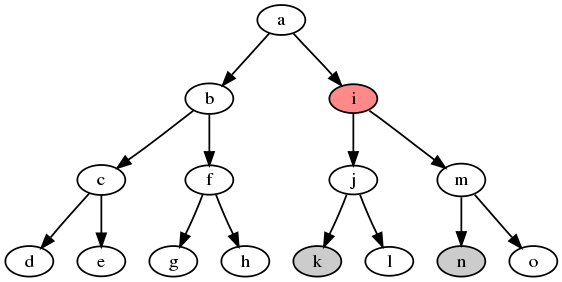
\includegraphics[width=0.50\textwidth]{LCA.png}
\caption{Node \textbf{$i$} is the least common ancestor of \textbf{$k$} and \textbf{$n$}.}
\end{figure}

To calculate the least common ancestor of nodes in our segmented tree we start by labeling each node using an in-order traversal.  The labeling is done in red in the figure below.

Then we proceed by comparing the binary representation of the nodes in question.

\begin{figure}[h]
\centering
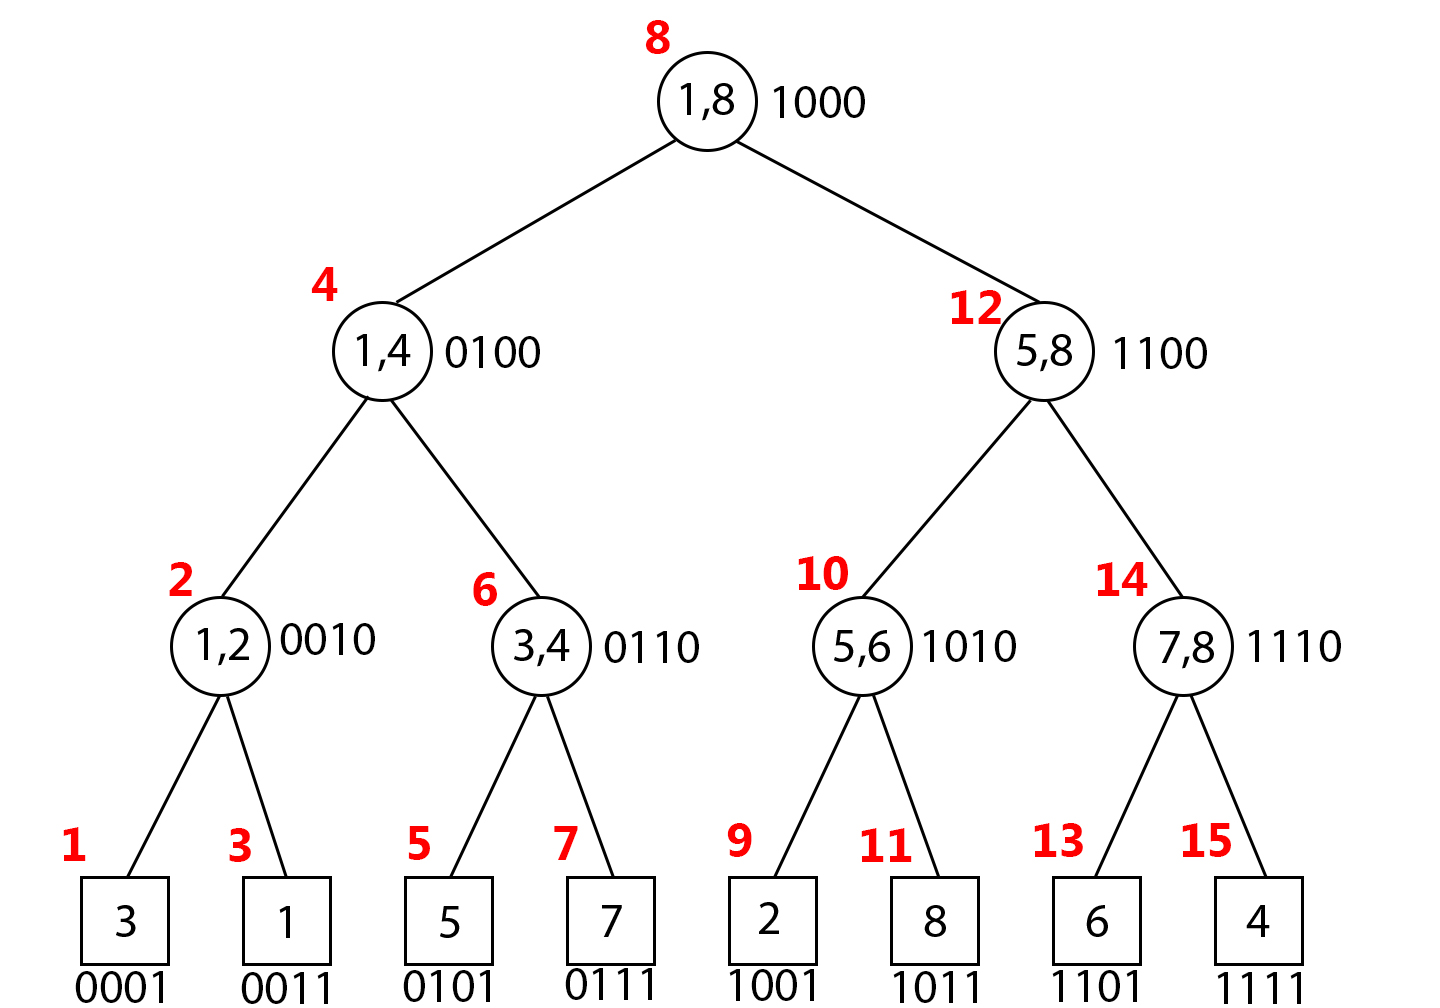
\includegraphics[width=0.75\textwidth]{tree2.jpg}
\caption{Calculating the least common ancestor using binary representation}
\end{figure}

The least common ancestor of nodes $A$ and $B$ is node $C$ and can be computed by comparing the binary representation of $A$ and $B$.

\begin{enumerate}
\item Compare $A$ and $B$ in bit-wise fashion starting from the left (most significant bit).
\item For a given bit position, if the bit in $A$ and $B$ match, then $C$ gets that value for that position.
\item Continue until you reach the first position where the bit in $A$ is not equal to the bit in $B$.  Set that position in $C$ to 1.
\item Set all subsequent positions in $C$ to 0.
\end{enumerate}

For example:

The first position in $A$ and $B$ match so the output $C$ gets the same value.  The second position differs so set that position in $C$ gets set to 1.  All subsequent values in $C$ are set to 0.

\begin{figure}[h]
  \begin{center}
    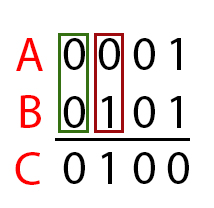
\includegraphics[width=0.2\textwidth]{bits.jpg}
  \end{center}
\end{figure}

The least common ancestor of nodes 1 (0001) and 5 (0101) is 4 (0100).

\hspace{5pt}

{\large \textbf{Putting It All Together: Using Segmented Tree to Calculate RMQ}}

We have generate a segmented tree, filled it with $P$ and $S$ arrays, and numbered the nodes using in-order traversal.  We still need to compute the range minimum query.

The steps to compute the $RMQ_{A}(i,j)$ are as follows:

\begin{enumerate}
    \item Find the \textbf{least common ancestor} of leaf nodes $i$ and $j$.  For example if $RMQ_{A}(2,3)$ then the internal node labeled "1,4" would be the least common ancestor of the leaf nodes 2 and 3.
    \item If the answer can be determined from that node we are done. Otherwise, use the suffix minima array from left child and the prefix minima array from the right child to compute the answer.
\end{enumerate}

Using \textbf{figure 22.3} as an example we are going to compute $RMQ_{A}(3,5)$:

The least common ancestor of the third and fifth leaf node is the root node.  But the answer cannot be determined from the root node itself so we must examine its children.  Using the $S$ = [1,1,5,7] from the left child and $P$ = [2,2,2,2] from the right child, we calculate $min(S[3], S[4], P[1]) = min(5, 7, 2) = 2$. 

$S[3], S[4],$ and $P[1]$ correspond to the indices (3,5) in the range minima query.



\section{Tree Contraction}

An expression can be represented by an expression tree where all leaf nodes are constants and all the internal nodes are operators.  Solving the expression tree iteratively can be inefficient for large or unbalanced trees.

\begin{figure}[h]
  \begin{center}
    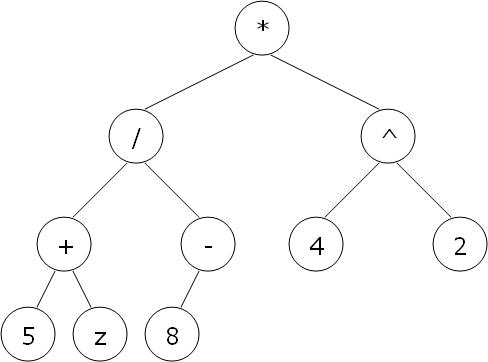
\includegraphics[width=0.4\textwidth]{exptree.JPG}
  \end{center}
  \caption{An expression tree}
\end{figure}


%\newpage

\subsection{\texttt{Rake} operation}

In order to solve the tree contraction problem efficiently we need to introduce the \texttt{rake} operation.

Let $T=(V,E)$ be a rooted binary tree for each vertex $v, P(v)$ is its parent.  $sib(v)$ is the child of $p(v)$.

The \texttt{rake} operation does the following:
\begin{enumerate}
  \item Removes $u$ and $p(u)$ from $T$, and
  \item Connects $sib(u)$ to $p(p(u))$
\end{enumerate}

\begin{figure}[h]
  \begin{center}
    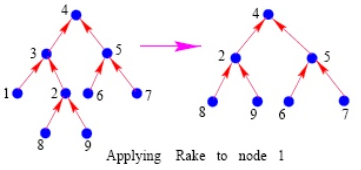
\includegraphics[width=0.5\textwidth]{rake.jpg}
  \end{center}
\end{figure}

\newpage
\subsection{Algorithm} 

In our tree contraction algorithm, we must apply the rake operation repeatedly to reduce the size of the binary tree.

We first label the leaves consecutively from left to right.  We exclude the leftmost and rightmost leaves.  These two leaves will be the two children of the root when the tree is contracted to a three-node tree.

\vspace{10pt}

\texttt{Tree Contraction Algorithm}

\hspace{10pt} \texttt{INPUT:} Rooted binary tree $T$.

\hspace{10pt} \texttt{OUTPUT:} 3-node binary tree

\begin{enumerate}
    \item We first label the leaves consecutively from left to right.  We exclude the leftmost and rightmost leaves.  These two leaves will be the two children of the root when the tree is contracted to a three-node tree.  Store all $n$ leaves in array $A$.  ($A_{odd}$ is the subarray consisting of the odd-indexed elements of $A$.  $A_{even}$ is the subarray consisting of the even-indexed elements of $A$.)
    \item For $i:=1$ to $log(n+1) \ \textbf{do}:$
        \begin{enumerate}
            \item Apply \texttt{rake} operation concurrently to each element of $A_{odd}$ that are left children.
            \item Apply \texttt{rake} operation concurrently to the rest of elements in $A_{odd}$.
            \item Set $A:=A_{even}$.
        \end{enumerate}
\end{enumerate}


\begin{figure}[h]
  \begin{center}
    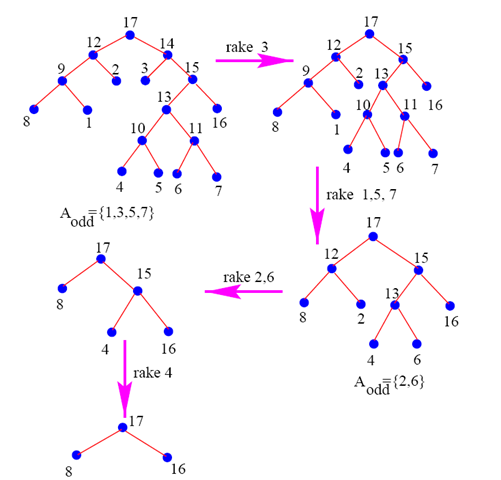
\includegraphics[width=0.4\textwidth]{finalrake.png}
  \end{center}
  \caption{Tree contraction using \texttt{rake} operator}
\end{figure}





\end{document}